\chapter{Introduction to NoSQL Injection}

\section{From SQL to NoSQL Injection}

\section{Definition of NoSQL Injection}
\subsection{Common Attacker Model}

\begin{figure}[h]
\centering
  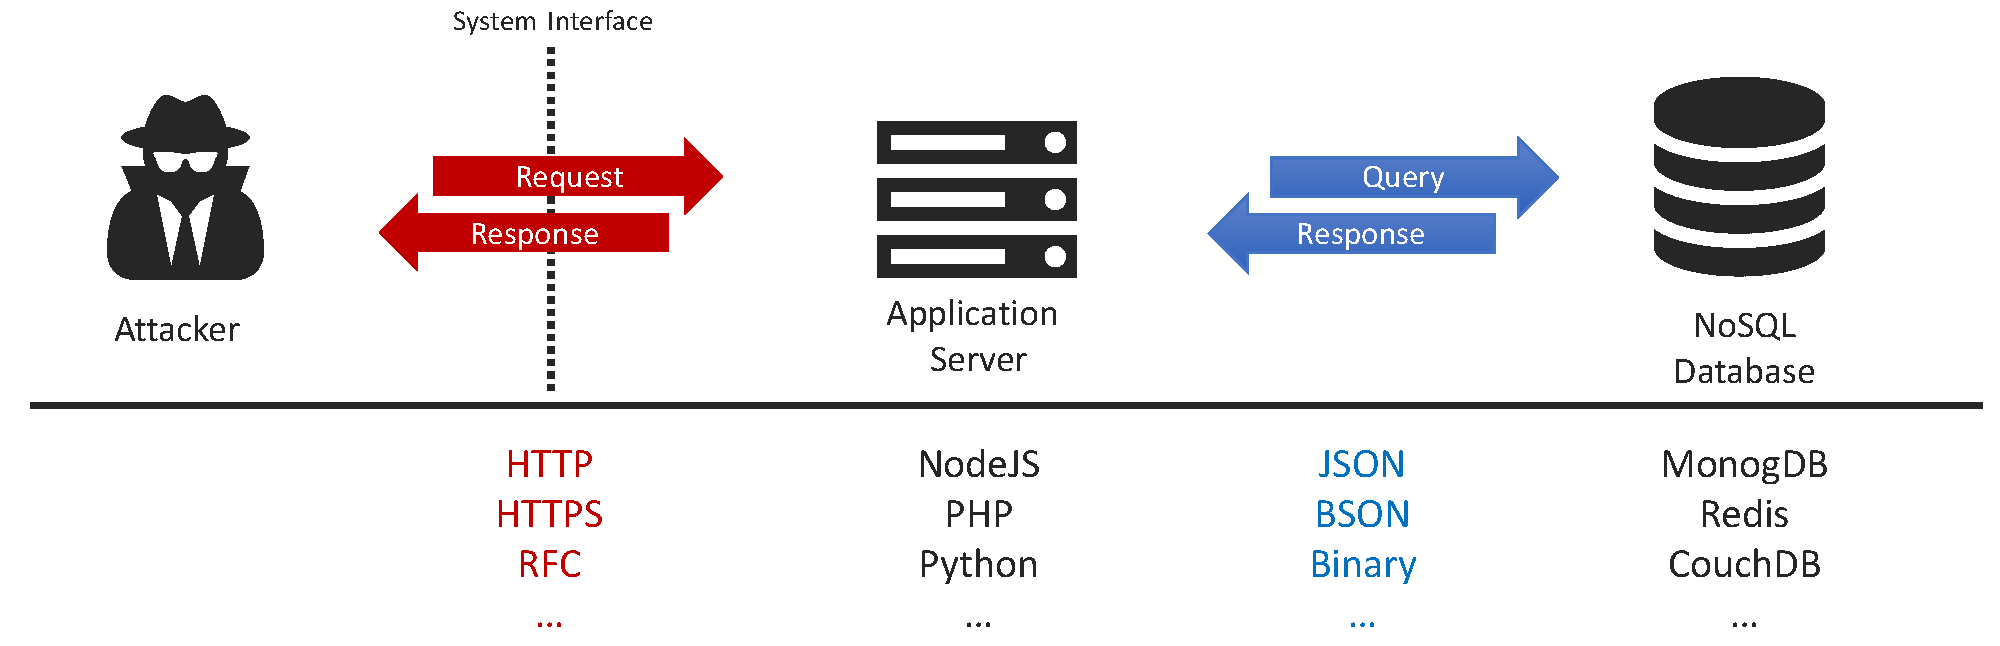
\includegraphics[width=1\linewidth]{Images/attacker_model_normal}
  \caption{Common attacker model for NoSQL injection}
  \label{fig:normalAttackerModel}
\end{figure}

% Objective

\subsection{Extended Attacker Model}

\begin{figure}[h]
\centering
  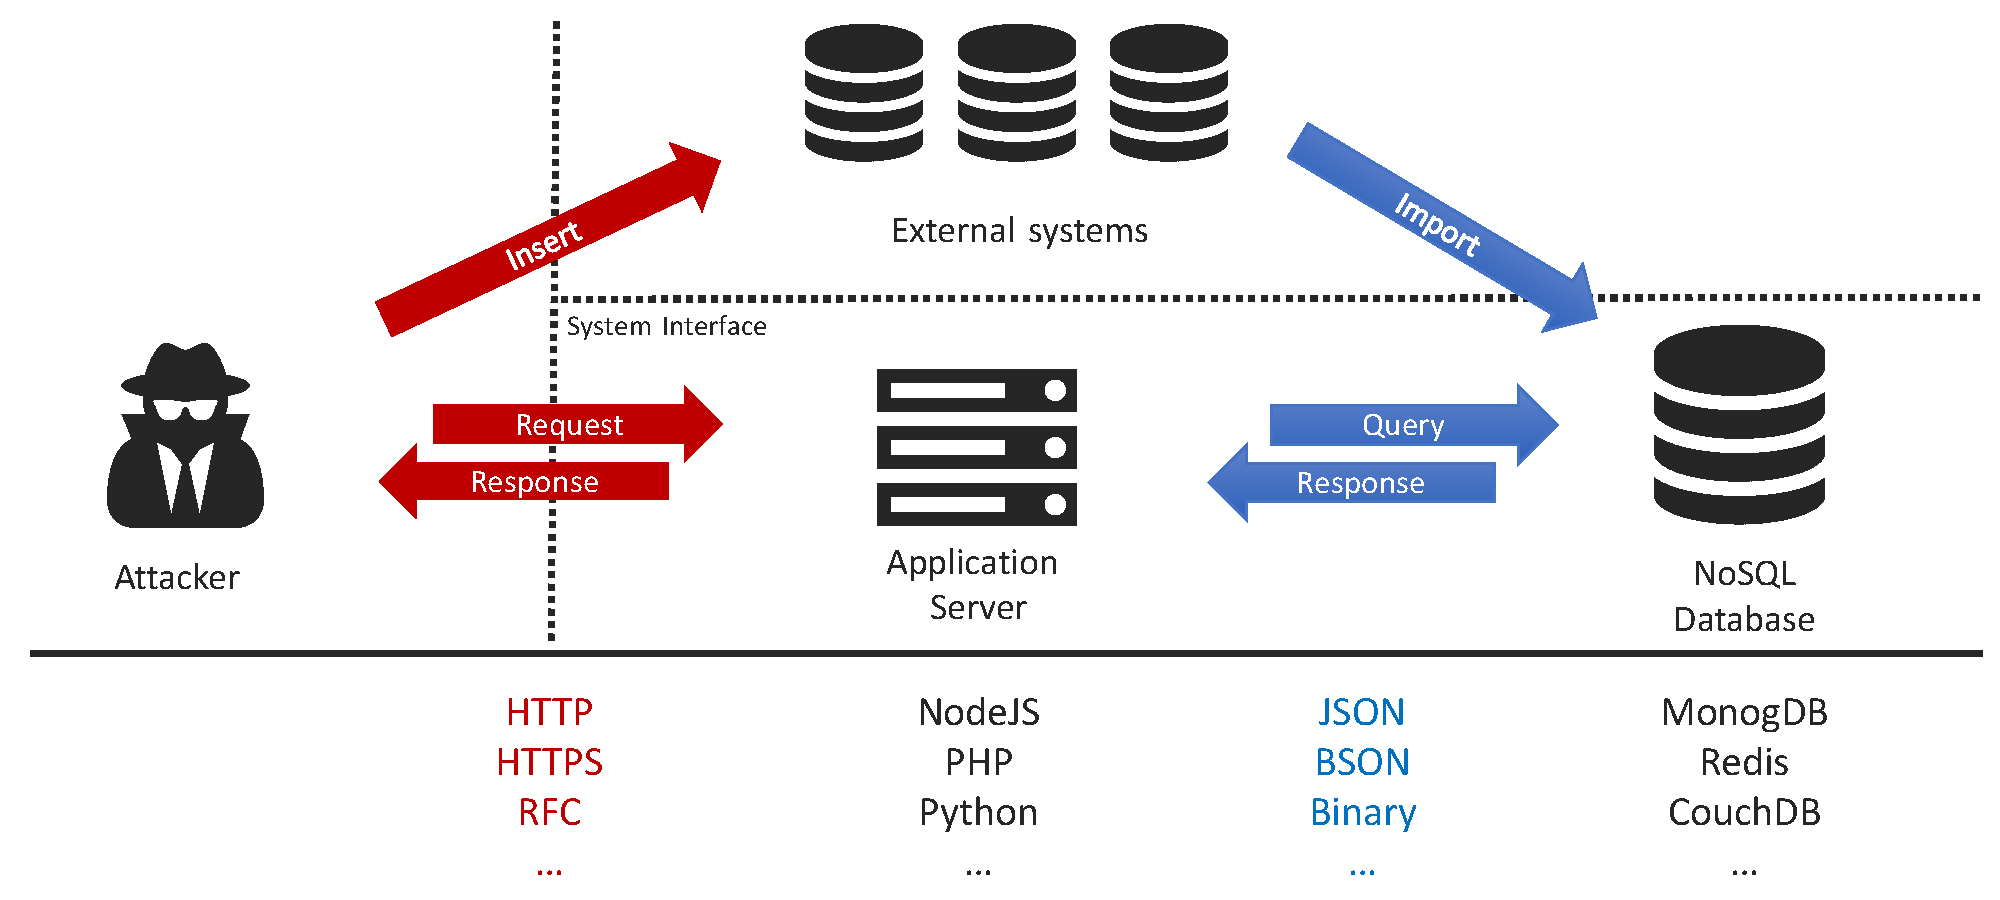
\includegraphics[width=1\linewidth]{Images/attacker_model_extended}
  \caption{Extended attacker model for NoSQL injection}
  \label{fig:extendedAttackerModel}
\end{figure}

% Objective

\subsection{Direct Attacker Model}

\begin{figure}[h]
\centering
  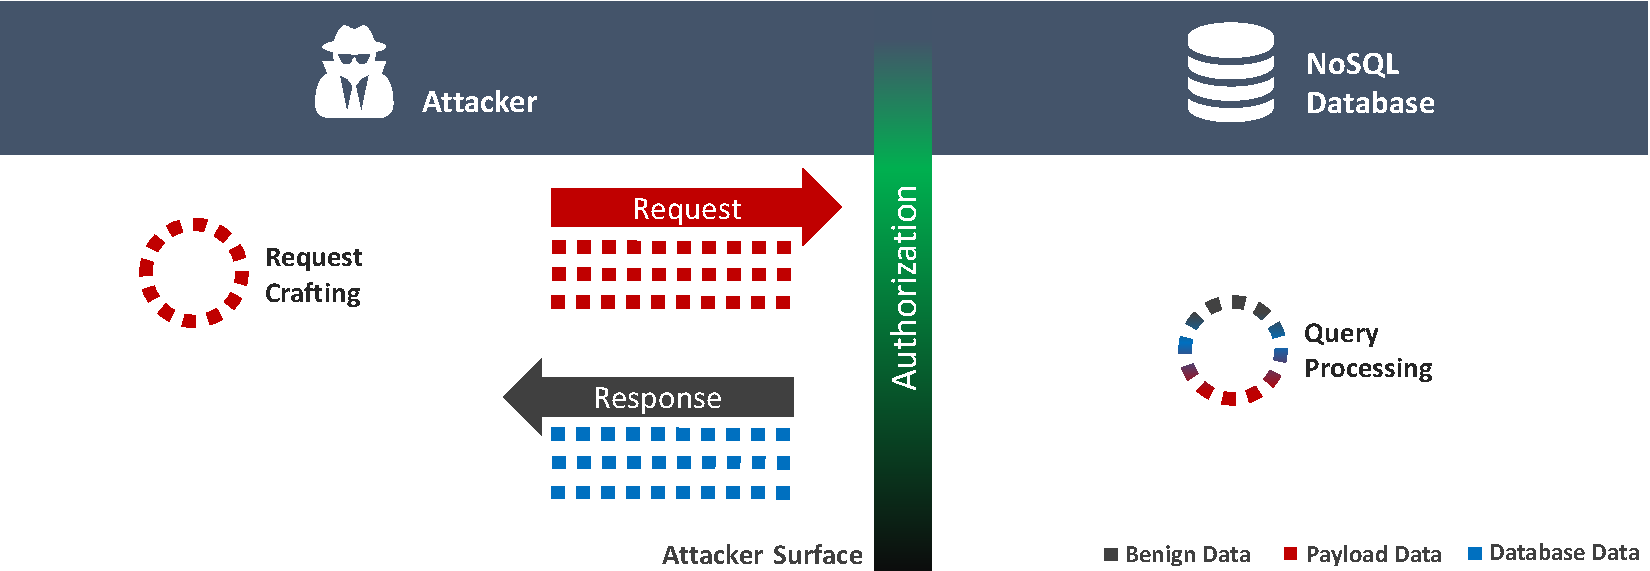
\includegraphics[width=1\linewidth]{Images/attacker_model_direct}
  \caption{Direct attacker model for NoSQL injection}
  \label{fig:extendedAttackerModel}
\end{figure}

% Objective


\section{Considered Technology Stack}
\subsection{Selected Databases}
\subsection{Selected Application Platforms}


\chapter{NoSQL Injection Attacks}

\section{MongoDB Document Store}
\subsection{Node.js Type Injection Attack}
\subsection{PHP Type Injection Attack}

\begin{lstlisting}[caption={Vulnerable PHP - MongoDb application}, label={lst:PHPArrayInjection}]
$collection->find(array('user' => $_GET['user'], 'password' => $_GET['password']));
\end{lstlisting}


\begin{lstlisting}[caption={MongoDB injection with PHP's associative arrays}, label={lst:PHPArrayInjection}]
https://example.org?user=patrick&password[%24ne]=1
\end{lstlisting}

\begin{lstlisting}[caption={Injected query parameter for MongoDB PHP injection}, label={lst:PHPArrayParam}]
{'user': 'patrick', 'password': {'&ne':1}}
\end{lstlisting}


\section{Redis Key-Value Store}
\subsection{Node.js Type Injection Attack}
\subsection{PHP Type Injection Attack}

\section{CouchDB Document Store}
\subsection{MapReduce Attack}